\documentclass[10pt]{article}
\usepackage{tmlr}
% \usepackage[preprint]{tmlr}  % for arxiv

\usepackage{amsmath,amssymb,amsthm}
\usepackage{hyperref}
\usepackage{url}
\usepackage{booktabs}
\usepackage{graphicx}
\usepackage{xcolor}
\usepackage{subcaption}

\newtheorem{proposition}{Proposition}
\newtheorem{corollary}{Corollary}
\newcommand{\todo}[1]{\textcolor{red}{[#1]}}
\newcommand{\E}{\mathbb{E}}
\newcommand{\KL}{\mathrm{KL}}
\newcommand{\Ts}{T^{*}}

\title{Weaker Language Models Need Colder Sampling,\\and Their Loss Says How Much}

\author{\name Anonymous authors \email anonymous@anonymous.org}

\def\month{MM}
\def\year{YYYY}
\def\openreview{\url{https://openreview.net/forum?id=XXXX}}

\begin{document}

\maketitle

\begin{center}
\fbox{\parbox{0.9\linewidth}{\small\textbf{Draft.} Every number in this version comes from a pilot run on WikiText-103 with a Qwen2.5-3B judge (Section~\ref{sec:setup}). A replication on text written in 2026 with a stronger judge, plus a direct measurement of the self-consistent temperature, is in progress. Red text marks what changes when it finishes.}}
\end{center}

\begin{abstract}
Most people sample every language model at a temperature of 0.7 or 1.0. We ask what temperature a given model actually needs. We define $\Ts$ as the temperature at which a model's samples are exactly as surprising to a stronger judge model as human-written text, and measure it for 14 base models from 70M to 2.8B parameters, including checkpoints from partway through training. $\Ts$ ranges from 0.62 to 0.83. It is set by the model's loss, not its size: two models with the same loss and a 3.5$\times$ difference in parameters have the same $\Ts$, and a two-number formula fitted on Pythia alone predicts the three SmolLM2 models to within 0.014. This looks like it contradicts recent work showing that the temperature which makes a model \emph{self-consistent} is the same at every scale. It doesn't. We prove that any model whose log loss cannot be improved by rescaling its logits is self-consistent at temperature 1, however bad it is, so self-consistency cannot see model quality. Only a reference outside the model can. Against such a reference, the extra surprise of a model's samples at temperature 1 is exactly the symmetric KL divergence between model and truth, roughly twice the model's excess loss, and a first-order expansion turns that into a prediction for $\Ts$ that matches simulation. Every experiment ran on a single 16GB laptop.
\end{abstract}

\section{Introduction}
\label{sec:intro}

We finetuned a 297M-parameter model to chat and asked it the capital of Australia. At temperature 0.7 it said Melbourne. On another try it said Perth. At 0.7 it gave a sensible reply to ``hi'' 8 times out of 12; at 0.4 it managed 12 out of 12. Lowering the temperature didn't make the model know more, but it stopped it from wandering into the parts of its distribution it had no business being in.

The usual advice is to pick a temperature between 0.7 and 1.0 and move on. That advice comes from large models. Nobody tells you what temperature a 70M or a 300M model wants, or what decides it. There is a large literature on \emph{how} to sample: top-$k$~\citep{fan2018hierarchical}, nucleus~\citep{holtzman2020curious}, typical~\citep{meister2023typical}, $\eta$~\citep{hewitt2022truncation} and min-$p$~\citep{nguyen2024minp} sampling all reshape the distribution before drawing from it. Much less work asks how the right setting should change from one model to the next.

The closest recent answer points the other way. \citet{cao2025entropy} show that language models become \emph{entropy-miscalibrated} as they generate (their per-step entropy drifts above their log loss) and that this barely improves with scale, so the temperature that fixes it is about the same from 0.5B to 72B parameters. If that were the whole story, one temperature would suit every model.

Our measurements say otherwise. We define the best temperature $\Ts$ as the one where a model's samples are as surprising to a stronger judge model as real human text is, and measure it for 14 base models. It moves from 0.62 to 0.83, and it moves with loss (Figure~\ref{fig:main}).

The two findings fit together once you separate two questions. ``Is the model consistent with itself?'' and ``does the model match the world?'' have different answers, and only the second one depends on how good the model is.

\paragraph{Contributions.}
\begin{itemize}
    \item \textbf{A measurement.} $\Ts$ for 14 base models from three families (Pythia, SmolLM2 and a 297M model we trained), 70M to 2.8B parameters, including Pythia checkpoints from partway through training (Section~\ref{sec:results}).
    \item \textbf{Loss, not size.} $\Ts$ is predicted by the model's loss ($r^2 = 0.95$); adding parameter count to the fit changes nothing. Two models with equal loss and a 3.5$\times$ size gap have equal $\Ts$. A fit on Pythia alone predicts SmolLM2 to within 0.014.
    \item \textbf{Why self-consistency can't see this.} A short proof that log-loss training makes any model self-consistent at temperature 1 regardless of quality, and an exact expression for how surprising its samples look to an outside reference: the symmetric KL divergence between model and truth (Section~\ref{sec:theory}).
    \item \textbf{A first-order formula} for $\Ts$ in terms of the loss gap, checked against simulation.
    \item \textbf{Everything on a laptop.} All runs used one 16GB MacBook Air. Code, generations and results are released.
\end{itemize}

\begin{figure}[t]
\centering
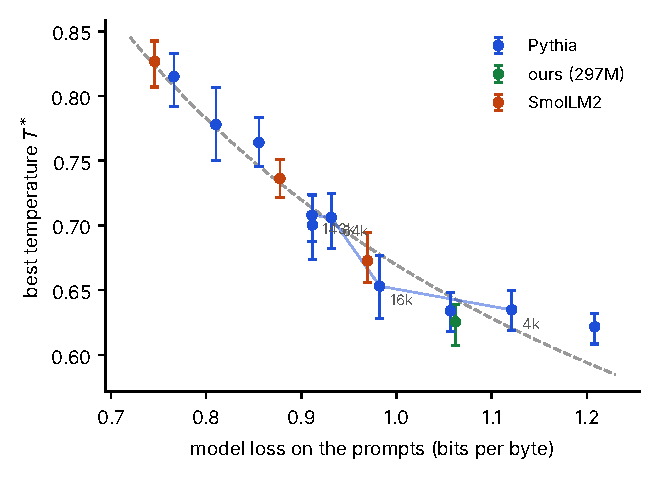
\includegraphics[width=0.62\linewidth]{figs/tstar_loss.pdf}
\caption{The best sampling temperature $\Ts$ against model loss for 14 base models. Error bars are 95\% bootstrap intervals over prompts. The dashed curve is $\Ts = 0.217 + 0.591\,h/L$, where $L$ is the model's loss and $h$ is the judge's loss on human text. The thin line joins four checkpoints of Pythia-410M, labelled by training step. Lower loss means a hotter best temperature, for every family.}
\label{fig:main}
\end{figure}

\section{Background and related work}
\label{sec:related}

\paragraph{Temperature and truncation.} Sampling at temperature $T$ draws from $q_T(y) \propto q(y)^{1/T}$. Below 1 it sharpens the distribution, above 1 it flattens it. Truncation methods~\citep{fan2018hierarchical,holtzman2020curious,meister2023typical,hewitt2022truncation,nguyen2024minp} cut off the low-probability tail instead of reweighting it. \citet{hewitt2022truncation} frame the tail as smoothing the model adds to avoid infinite loss, which is close to how we think about temperature here. \citet{finlayson2024closing} trace tail errors to the softmax bottleneck. We study plain temperature because it has one parameter, which makes ``what value does this model need'' a well-posed question.

\paragraph{Picking the temperature.} Mirostat~\citep{basu2021mirostat} adjusts truncation while decoding to hold perplexity at a target. That is the closest idea to ours, but it needs the target chosen by hand and does not say how the target should depend on the model. \citet{li2025hot} find that larger models tolerate higher temperatures before benchmark scores drop, which agrees with our direction. \citet{du2025optimizing} choose temperature for multi-sample reasoning, and \citet{zhu2024hot} adapt it per token for code. None of these relate the temperature to the model's loss.

\paragraph{Entropy calibration.} \citet{braverman2020calibration} showed that the entropy of generated text drifts upward over long generations, and that a model's entropy rate can be calibrated against its log loss. \citet{cao2025entropy} show that this miscalibration shrinks very slowly with scale, explain it with a power-law model of rare tokens, and find that the temperature giving zero calibration error is similar across model sizes. Our results agree with theirs. We argue they answer a different question from ours (Section~\ref{sec:theory}).

\paragraph{Calibration and scaling.} Temperature scaling is the standard fix for overconfident classifiers~\citep{guo2017calibration}. Scaling laws relate loss to parameters and data~\citep{kaplan2020scaling,hoffmann2022training}. Our result adds a decoding-side quantity that follows loss rather than parameters.

\section{Three ways to define the right temperature}
\label{sec:defs}

Let $p(\cdot \mid c)$ be the true next-token distribution after context $c$, and let the model have logits $\ell(c)$ and distribution $q(\cdot \mid c) = \mathrm{softmax}(\ell(c))$. Sampling at temperature $T$ uses $q_T = \mathrm{softmax}(\ell / T)$. Write $H = \E_c\, \mathrm{H}(p(\cdot \mid c))$ for the entropy of the truth and $L = \E_c \E_{y \sim p}[-\log q(y \mid c)]$ for the model's loss. Three temperatures are worth naming.

\paragraph{Best for log loss, $T_{\text{cal}}$.} The $T$ that minimises $\E_c \E_{y\sim p}[-\log q_T(y \mid c)]$. This is classic temperature scaling~\citep{guo2017calibration}.

\paragraph{Self-consistent, $T_{\text{self}}$.} The $T$ at which the model's entropy equals its log loss, $\E_c\, \mathrm{H}(q_T) = \E_c \E_{y\sim p}[-\log q_T(y \mid c)]$. This is entropy calibration~\citep{braverman2020calibration,cao2025entropy}. A self-consistent model is exactly as surprised by its own samples as by real text.

\paragraph{Matches the world, $\Ts$.} The $T$ at which the model's samples are as surprising \emph{to the truth} as real text is: $\E_c \E_{y \sim q_T}[-\log p(y \mid c)] = H$. In practice we cannot evaluate $p$, so we use a judge model $J$ much stronger than the models being tested, and compare the judge's bits per byte on samples against its bits per byte on human continuations of the same prompts.

$T_{\text{self}}$ only involves the model. $\Ts$ needs something outside it. That difference turns out to be the whole story.

\section{Why self-consistency can't see model quality}
\label{sec:theory}

We work one step at a time: contexts come from real text and we look at the next token. Section~\ref{sec:accumulation} discusses what changes over a whole generation.

\begin{proposition}[Log-loss training gives self-consistency for free]
\label{prop:self}
Let $q_\beta = \mathrm{softmax}(\beta \ell)$ and suppose $\beta^{*}$ minimises the log loss $\Lambda(\beta) = \E_c \E_{y\sim p}[-\log q_\beta(y \mid c)]$. Then at $\beta^{*}$ the model's average entropy equals its log loss:
\[
\E_c\, \mathrm{H}(q_{\beta^{*}}) = \Lambda(\beta^{*}).
\]
\end{proposition}

\begin{proof}
Write $Z_\beta(c) = \sum_y e^{\beta \ell_y(c)}$, so $-\log q_\beta(y \mid c) = -\beta \ell_y(c) + \log Z_\beta(c)$. Then
\[
\Lambda(\beta) = \E_c\!\left[-\beta\, \E_{p}[\ell] + \log Z_\beta\right], \qquad
\E_c\, \mathrm{H}(q_\beta) = \E_c\!\left[-\beta\, \E_{q_\beta}[\ell] + \log Z_\beta\right].
\]
Since $\tfrac{d}{d\beta} \log Z_\beta = \E_{q_\beta}[\ell]$, we get $\Lambda'(\beta) = \E_c[\E_{q_\beta}[\ell] - \E_p[\ell]]$. $\Lambda$ is convex in $\beta$, so at the minimum $\E_c \E_{q_{\beta^*}}[\ell] = \E_c \E_p[\ell]$. Subtracting the two lines above at $\beta^*$ gives $\E_c\, \mathrm{H}(q_{\beta^*}) - \Lambda(\beta^*) = -\beta^*\left(\E_c\E_{q_{\beta^*}}[\ell] - \E_c\E_p[\ell]\right) = 0$.
\end{proof}

A network trained with log loss can rescale its own logits through its final layer, so in practice $\beta^* \approx 1$, and the proposition says $T_{\text{self}} = T_{\text{cal}} = 1$ for one step. Nothing in the proof depends on how close $q$ is to $p$. A model that is badly wrong is still self-consistent, because it is wrong about the world in the same way it is wrong about its own samples.

Now look at the same model from outside.

\begin{corollary}[What an outside reference sees]
\label{cor:jeffreys}
Under the conditions of Proposition~\ref{prop:self} with $\beta^* = 1$, the extra surprise of the model's samples to the truth, at temperature 1, is the symmetric KL divergence between truth and model:
\[
\E_c \E_{y\sim q}[-\log p(y \mid c)] - H \;=\; \E_c\left[\KL(p \,\|\, q) + \KL(q \,\|\, p)\right].
\]
\end{corollary}

\begin{proof}
$\E_{q}[-\log p] = \mathrm{H}(q) + \KL(q\|p)$. By Proposition~\ref{prop:self}, $\E_c \mathrm{H}(q) = L = H + \E_c \KL(p\|q)$. Substitute.
\end{proof}

So unless the model is perfect, its samples at $T = 1$ are too surprising, and $\Ts < 1$. The excess is at least the model's excess loss $L - H = \E_c \KL(p\|q)$, and for small errors the two KL terms are about equal, so the excess is roughly twice the loss gap. Lowering $T$ reduces it. Expanding the judged surprise to first order around $T = 1$, using $\tfrac{d}{dT}\E_{q_T}[f]\big|_{T=1} = \mathrm{Cov}_q(\log q, -f)$, gives
\begin{equation}
\Ts \;\approx\; 1 - \frac{\E_c\left[\KL(p\|q) + \KL(q\|p)\right]}{\E_c\, \mathrm{Cov}_{q}(\log q, \log p)} \;\approx\; 1 - \frac{2\,(L - H)}{C},
\label{eq:firstorder}
\end{equation}
where $C$ measures how spread out the log-probabilities are (for a good model, close to the variance of $\log p$, sometimes called varentropy). Worse loss, lower $\Ts$, at a rate set by how varied the text is.

\paragraph{A toy model.} We checked this with a simulation (Figure~\ref{fig:toy}). The truth is 1{,}500 Zipf-shaped next-token distributions over 4{,}000 tokens with random steepness. A model of quality $\sigma$ has logits $\log p + \sigma \varepsilon$ with Gaussian noise $\varepsilon$, rescaled by the log-loss-optimal temperature, which is what training would do. As $\sigma$ grows, $T_{\text{cal}}$ and $T_{\text{self}}$ stay at exactly 1.000, as Proposition~\ref{prop:self} says they must. $\Ts$ falls from 1.0 to 0.47. The excess surprise at $T = 1$ matches the symmetric KL to four decimal places, and Equation~\ref{eq:firstorder} predicts $\Ts$ to within 0.003 for loss gaps up to 7\% of $H$ and within 0.02 at 17\%. Plotted against $H/L$, $\Ts$ is close to a straight line ($r^2 = 0.98$), the same form that fits our real models best (Section~\ref{sec:results}).

\begin{figure}[t]
\centering
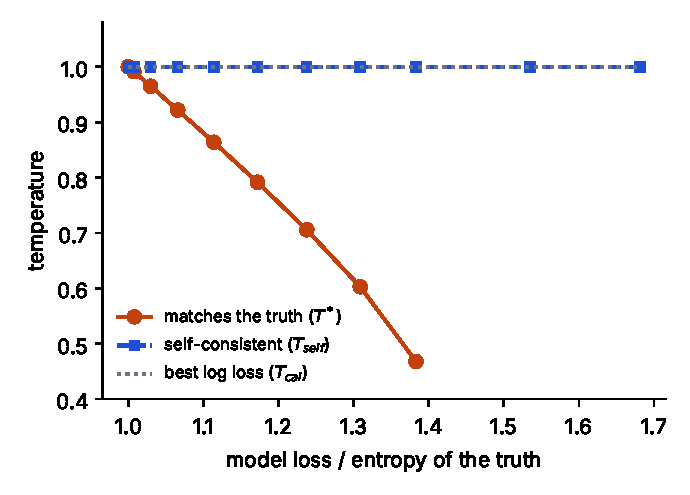
\includegraphics[width=0.55\linewidth]{figs/toy.pdf}
\caption{Toy model. Models get worse to the right. The log-loss-optimal temperature and the self-consistent temperature stay at 1 for every model (Proposition~\ref{prop:self}). The temperature that matches the truth falls steadily as the model gets worse.}
\label{fig:toy}
\end{figure}

\subsection{Over a whole generation}
\label{sec:accumulation}

Real generations feed the model its own samples as context, and errors pile up: this is the entropy drift of \citet{braverman2020calibration} and \citet{cao2025entropy}. It pushes every model's measured $T_{\text{self}}$ below 1, by an amount that barely depends on scale. It also pushes $\Ts$ below the one-step value. Together, the theory predicts:

\begin{enumerate}
    \item \textbf{P1.} $T_{\text{cal}} \approx 1$ for every model.
    \item \textbf{P2.} $T_{\text{self}}$ below 1 and roughly flat across models, as in \citet{cao2025entropy}.
    \item \textbf{P3.} $\Ts$ below $T_{\text{self}}$ for weak models, rising toward it as loss falls.
    \item \textbf{P4.} $\Ts$ measured on the second half of a continuation lower than on the first half, by a similar amount for every model.
    \item \textbf{P5.} Text sampled at $\Ts$ preferred over text at the default temperatures.
\end{enumerate}

\todo{P1, P2 and P4 are measured directly in the full run (the script now records the model's loss at 25 temperatures, its surprise at its own samples, and judge scores for each half of the continuation). P5 is the preference study in Section~\ref{sec:limits}.}

\section{Setup}
\label{sec:setup}

\paragraph{Text.} 200 passages from WikiText-103~\citep{merity2016pointer}. Each gives a 40-word prompt and the next 80 words as the human continuation. \todo{Full run: 300+ passages per model from English Wikipedia articles created in 2026, after every model's training cutoff.}

\paragraph{Models.} Pythia 70M, 160M, 410M, 1B, 1.4B and 2.8B~\citep{biderman2023pythia}; Pythia-410M at training steps 4k, 16k and 64k and Pythia-1.4B at step 16k; SmolLM2 135M, 360M and 1.7B~\citep{allal2025smollm2}; and a 297M Llama-style model we pretrained on 6.1B tokens. Pythia runs in fp32 (fp16 for 2.8B) because it breaks in bf16: on a test paragraph Pythia's loss went from 4.15 to 5.90. \todo{Full run adds Pythia-160M at seven checkpoints from step 1k to 64k and Pythia-1B at 4k and 16k.}

\paragraph{Sampling.} Pure temperature sampling, no top-$k$ or top-$p$, 160 new tokens truncated to 80 words, temperatures 0.1 to 1.5 in steps of 0.1, fixed seeds. Each model generates for each prompt at every temperature.

\paragraph{Judge.} Qwen2.5-3B~\citep{qwen2025qwen25} scores every continuation in bits per byte given its prompt, so models with different tokenizers are comparable. It also scores the human continuations, giving the human level $h = 0.766$ bits per byte. \todo{Full run: Qwen2.5-7B, 4-bit, in MLX.}

\paragraph{Measuring $\Ts$ and $L$.} For each model, the judge's bits per byte rises with temperature (Figure~\ref{fig:curves}); $\Ts$ is where the curve crosses $h$, interpolated linearly between grid points. We bootstrap prompts 300 times for 95\% intervals. $L$ is the model's own bits per byte on the human continuations.

\paragraph{Compute.} One MacBook Air (M5, 16GB, no fan). The pilot ran overnight for 9.6 hours. Generation held about 345 tokens per second for Pythia-410M for the whole run, so the fanless chassis did not throttle it noticeably.

\section{Results}
\label{sec:results}

\subsection{Every model wants a temperature below 1}

Figure~\ref{fig:curves} shows the judge's bits per byte on each model's samples as temperature rises. At $T = 1$ every model is too surprising: from 1.05 bits per byte for SmolLM2-1.7B and Pythia-2.8B up to 1.67 for Pythia-70M, against 0.77 for human text. Every curve crosses the human line between 0.6 and 0.85. At the common default of 0.7, the six weakest models are too hot, the five best are too cold, and only the three in the middle have intervals that include 0.7.

\begin{figure}[t]
\centering
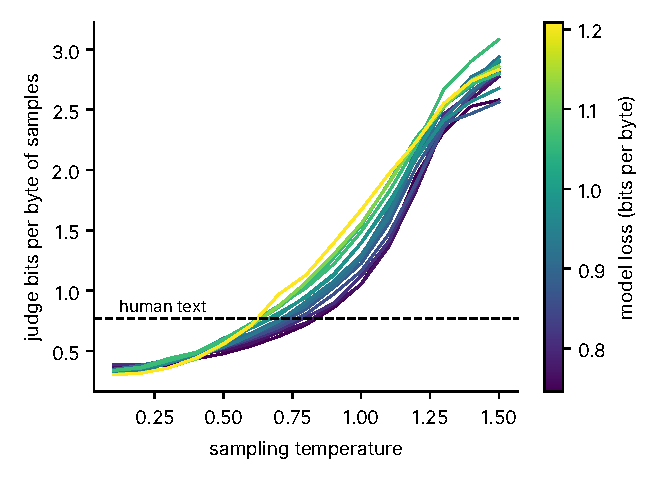
\includegraphics[width=0.55\linewidth]{figs/curves.pdf}
\caption{How surprising each model's samples are to the judge, by temperature. Colour is the model's loss. The dashed line is human text. Each model's $\Ts$ is where its curve crosses the line, and worse models cross earlier.}
\label{fig:curves}
\end{figure}

\subsection{Loss predicts $\Ts$}

Table~\ref{tab:models} lists all 14 models. $\Ts$ rises steadily as loss falls. Table~\ref{tab:fits} compares ways of predicting it. The best is linear in $h/L$:
\begin{equation}
\Ts \approx 0.217 + 0.591\,\frac{h}{L},
\label{eq:fit}
\end{equation}
with $r^2 = 0.955$ and a leave-one-out error of 0.014 on average (0.042 at worst). A straight line in $L$ does worse ($r^2 = 0.896$) because the relationship bends at both ends; the $h/L$ form is the one the toy model produces. Parameter count alone gets $r^2 = 0.68$.

\begin{table}[t]
\centering
\small
\begin{tabular}{lrrrcr}
\toprule
model & params & loss $L$ & $\Ts$ & 95\% interval & prompts \\
\midrule
SmolLM2-1.7B & 1711M & 0.746 & 0.827 & 0.807--0.842 & 100 \\
Pythia-2.8B & 2775M & 0.766 & 0.815 & 0.792--0.833 & 100 \\
Pythia-1.4B & 1415M & 0.810 & 0.778 & 0.750--0.806 & 100 \\
Pythia-1B & 1012M & 0.856 & 0.764 & 0.746--0.783 & 200 \\
SmolLM2-360M & 362M & 0.878 & 0.736 & 0.721--0.751 & 200 \\
Pythia-410M & 405M & 0.911 & 0.708 & 0.688--0.724 & 200 \\
Pythia-1.4B @ 16k & 1415M & 0.912 & 0.700 & 0.674--0.723 & 100 \\
Pythia-410M @ 64k & 405M & 0.932 & 0.706 & 0.682--0.725 & 100 \\
SmolLM2-135M & 135M & 0.970 & 0.673 & 0.656--0.695 & 200 \\
Pythia-410M @ 16k & 405M & 0.982 & 0.653 & 0.628--0.677 & 100 \\
Pythia-160M & 162M & 1.057 & 0.634 & 0.618--0.648 & 200 \\
ours-297M & 297M & 1.062 & 0.626 & 0.607--0.639 & 200 \\
Pythia-410M @ 4k & 405M & 1.121 & 0.635 & 0.619--0.650 & 200 \\
Pythia-70M & 70M & 1.208 & 0.622 & 0.608--0.632 & 200 \\
\bottomrule
\end{tabular}
\caption{All 14 models, sorted by loss (bits per byte on the human continuations). $\Ts$ is the judge-matched temperature. The judge's loss on human text is $h = 0.766$.}
\label{tab:models}
\end{table}

\begin{table}[t]
\centering
\small
\begin{tabular}{lccc}
\toprule
predictor & $r^2$ & leave-one-out error & worst \\
\midrule
$h / L$ & \textbf{0.955} & \textbf{0.014} & \textbf{0.042} \\
$\log L$ & 0.931 & 0.018 & 0.058 \\
$L$ & 0.896 & 0.023 & 0.075 \\
$L$ and $\log(\text{params})$ & 0.899 & & \\
$\log(\text{params})$ & 0.681 & 0.038 & 0.075 \\
\bottomrule
\end{tabular}
\caption{Linear predictors of $\Ts$ across 14 models. Adding parameters to loss raises $r^2$ by 0.003; its coefficient is 0.017 per factor of 10.}
\label{tab:fits}
\end{table}

\subsection{Size adds nothing once you know the loss}

Pythia-1.4B at step 16k and the finished Pythia-410M have the same loss (0.912 and 0.911) and 3.5$\times$ different parameter counts. Their $\Ts$ values are 0.700 and 0.708, inside each other's intervals. SmolLM2-135M and Pythia-410M at step 16k make a second pair: similar loss (0.970 and 0.982), 3$\times$ apart in size, $\Ts$ of 0.673 and 0.653. Regressing $\Ts$ on loss and $\log(\text{params})$ together gives the parameter term a coefficient of 0.017 per factor of ten and improves $r^2$ from 0.896 to 0.899. Figure~\ref{fig:size} shows both views.

\begin{figure}[t]
\centering
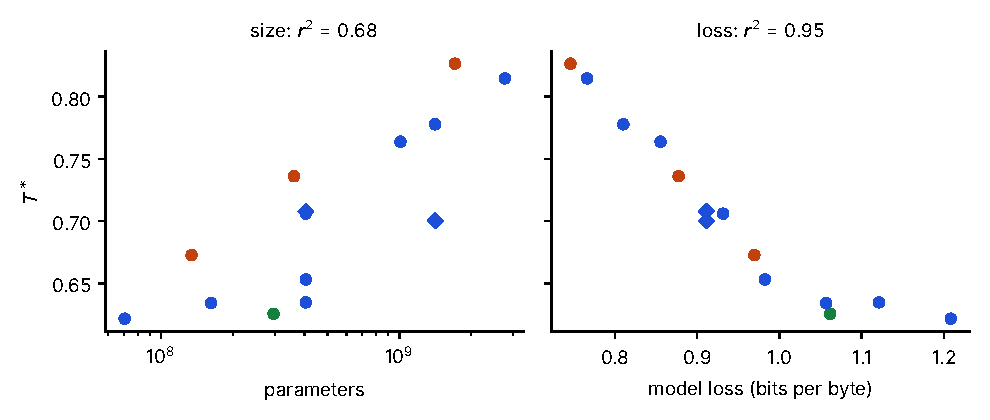
\includegraphics[width=0.85\linewidth]{figs/size_vs_loss.pdf}
\caption{$\Ts$ against parameters (left) and against loss (right). Diamonds are the matched pair Pythia-410M and Pythia-1.4B at step 16k: same loss, 3.5$\times$ different size, same $\Ts$.}
\label{fig:size}
\end{figure}

\subsection{Inside one training run}

The cleanest test holds the architecture fixed and lets only training change. Pythia-410M at steps 4k, 16k, 64k and 143k (the final model) has loss 1.121, 0.982, 0.932 and 0.911, and $\Ts$ of 0.635, 0.653, 0.706 and 0.708. The same network wants a hotter temperature as it learns, and it moves along the same curve as the other models (Figure~\ref{fig:main}). \todo{Full run: seven Pythia-160M checkpoints and two Pythia-1B checkpoints.}

\subsection{Across model families}

We fitted Equation~\ref{eq:fit} on the 10 Pythia models only and used it to predict the others (Table~\ref{tab:transfer}). It gets the three SmolLM2 models to within 0.014, all inside their bootstrap intervals. Our 297M model comes out 0.022 colder than predicted, just outside its interval. That model was trained on a different data mix with a different tokenizer, and we do not yet know whether the gap is real.

\begin{table}[t]
\centering
\small
\begin{tabular}{lcccc}
\toprule
model & predicted & measured & error & inside interval \\
\midrule
SmolLM2-1.7B & 0.821 & 0.827 & $+$0.006 & yes \\
SmolLM2-360M & 0.733 & 0.736 & $+$0.003 & yes \\
SmolLM2-135M & 0.686 & 0.673 & $-$0.014 & yes \\
ours-297M & 0.647 & 0.626 & $-$0.022 & no \\
\bottomrule
\end{tabular}
\caption{Fitted on Pythia only ($\Ts = 0.238 + 0.567\,h/L$), tested on the other families.}
\label{tab:transfer}
\end{table}

\subsection{A second check that didn't work}

We also looked for the temperature where the share of distinct words in a sample matches human text. It came out between 0.90 and 0.93 for every model, with no trend. Eighty words is too short for distinct-word counts to separate models, so we do not use this measure further.

\section{Using it}
\label{sec:using}

Equation~\ref{eq:fit} needs two numbers: your model's loss on some text it has not seen, and a strong model's loss on the same text. In our setting the rule of thumb is simple. Models around 1.2 bits per byte want about 0.62. Models around 0.9 want about 0.71. Models near the judge's own level want about 0.82. The usual 0.7 is close for mid-sized models and wrong at both ends: too hot for the small models people run on phones and laptops, and too cold for the best models we tested. The exact constants depend on the text domain and the judge, which is why the full run repeats everything with a second judge.

\section{Limitations}
\label{sec:limits}

\begin{itemize}
    \item \textbf{The judge is not much stronger than the best models.} SmolLM2-1.7B (0.746) beats Qwen2.5-3B on these prompts (0.766), and Pythia-2.8B ties it. The method assumes the judge knows real text better than the models it judges, so the top of the curve is the least reliable part. \todo{Full run uses Qwen2.5-7B.}
    \item \textbf{Contamination.} WikiText-103 is old Wikipedia, which appears in the Pile and so in Pythia's training data. That can make Pythia's loss look better than it is. \todo{Full run uses 2026 articles.} Fresh Wikipedia has its own problem: some new articles may have been drafted with language models, so ``human text'' is not guaranteed.
    \item \textbf{``Best'' is defined by the judge.} Matching the judge's surprise at human text is one definition of the right temperature. \todo{Planned: a pairwise preference test (an instruction-tuned judge picks the more natural of two continuations, order randomised, $\Ts$ against 0.7 and 1.0), plus 50 blind human pairs.}
    \item \textbf{Scope.} One domain (encyclopedia text), base models only, at most 2.8B parameters, 80-word continuations, plain temperature with no truncation. Chat models are tuned differently and may behave differently.
    \item \textbf{Few prompts for the largest models.} The four largest models have 100 prompts each, so their intervals are the widest.
    \item \textbf{The theory is one-step.} Propositions~\ref{prop:self} and~\ref{cor:jeffreys} describe next-token prediction from real contexts. Error accumulation over a generation is handled by citing \citet{cao2025entropy}, not derived.
\end{itemize}

\section{Conclusion}

The temperature that makes a model consistent with itself is the same for every model, and we proved it has to be: log-loss training guarantees it. The temperature that makes a model's text look like human text is different for every model, and it is set by how good the model is. Measure your model's loss on fresh text, and Equation~\ref{eq:fit} tells you roughly how cold to sample. Small models need it most.

\section*{Broader impact statement}

This work helps small models that run on personal devices produce more coherent text with no extra compute. We do not see a meaningful route to harm from choosing a sampling temperature.

\bibliography{refs}
\bibliographystyle{tmlr}

\appendix

\section{Proof of the first-order formula}
\label{app:firstorder}

Let $g(T) = \E_c \E_{y\sim q_T}[-\log p(y \mid c)]$. With $q_T \propto q^{1/T}$, $\tfrac{d}{dT}\E_{q_T}[f] = -\tfrac{1}{T^2}\mathrm{Cov}_{q_T}(\log q, f)$, so $g'(1) = \E_c\, \mathrm{Cov}_q(\log q, \log p)$, which is positive whenever model and truth broadly agree on which tokens are likely. Corollary~\ref{cor:jeffreys} gives $g(1) - H = \E_c[\KL(p\|q) + \KL(q\|p)]$. Solving $g(1) + (\Ts - 1)\,g'(1) = H$ gives Equation~\ref{eq:firstorder}. Since both KL terms equal $\tfrac12 \E \delta^2$ to second order in the log-probability error $\delta$, their sum is about $2(L - H)$.

In the simulation the predicted and true $\Ts$ were 0.991 and 0.991 at a 0.8\% loss gap, 0.965 and 0.965 at 3\%, 0.925 and 0.922 at 7\%, 0.872 and 0.864 at 11\%, and 0.811 and 0.792 at 17\%.

\section{Simulation details}
\label{app:sim}

Vocabulary 4{,}000, 1{,}500 contexts. Context $i$ has $p_i(k) \propto k^{-\alpha_i}$ over a ranking of tokens, with $\alpha_i$ uniform on $[0.9, 2.2]$, giving entropies from near zero to several nats ($H = 3.24$ nats on average). Model logits are $b(\log p + \sigma \varepsilon)$ with $\varepsilon$ standard Gaussian per token and context and $b$ chosen to minimise log loss. $\Ts$, $T_{\text{self}}$ and $T_{\text{cal}}$ are found by root finding and bounded minimisation. Code is in the supplement.

\section{Pythia in bfloat16}
\label{app:bf16}

Pythia was trained in fp16. Loading it in bf16 raised its loss on a test paragraph from 4.15 to 5.90. Every Pythia model here runs in fp32, except Pythia-2.8B in fp16 to fit in 16GB. The judge runs in bf16.

\section{Full curves}
\label{app:curves}

\todo{Per-model judge curves with intervals, and the human-level line, for every model in the full run.}

\section{Reproducing}
\label{app:repro}

\todo{One command to rebuild the prompts, one to run every model (it resumes where it stopped), one to make every table and figure. Hours per model on the laptop.}

\end{document}
